\section{Business Process Scheduling}
\label{sec:motivating}
\begin{figure*}[t]
    \centering
    \subfloat[\centering BPMN\label{fig:TPN}]{{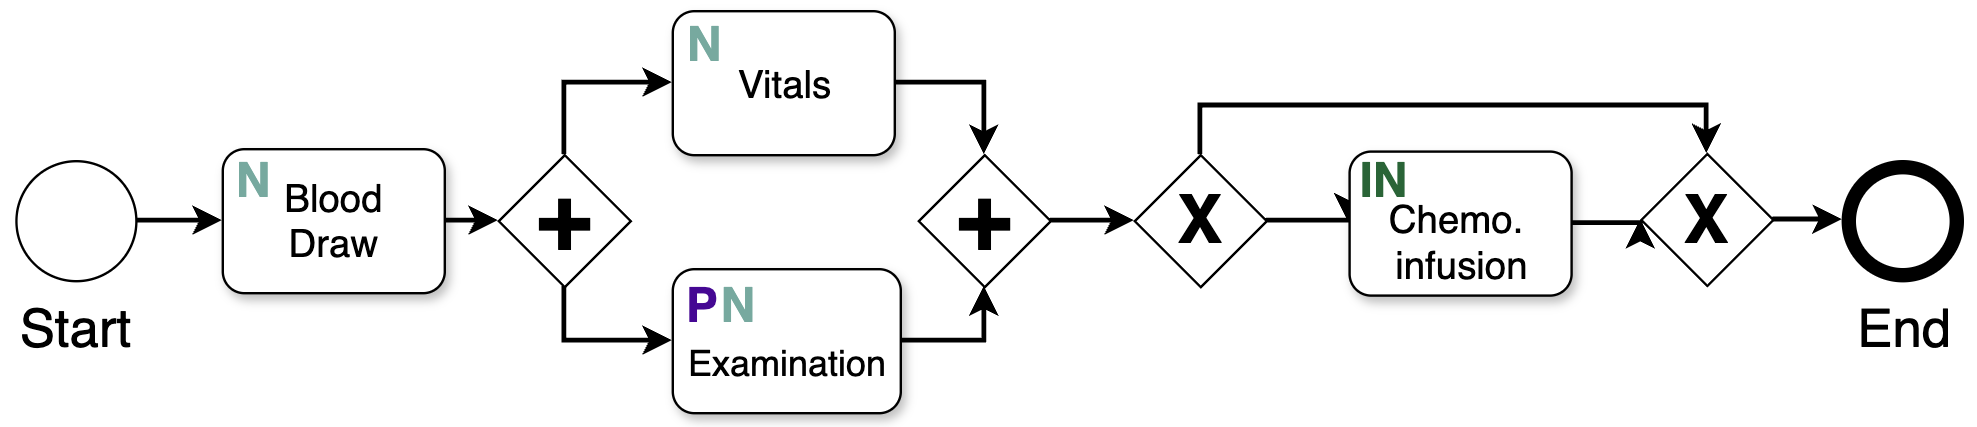
\includegraphics[width=0.75\textwidth]{images/bpmn.png} }}%
    \qquad
    \subfloat[\centering Resource calendars\label{fig:calendar}]{{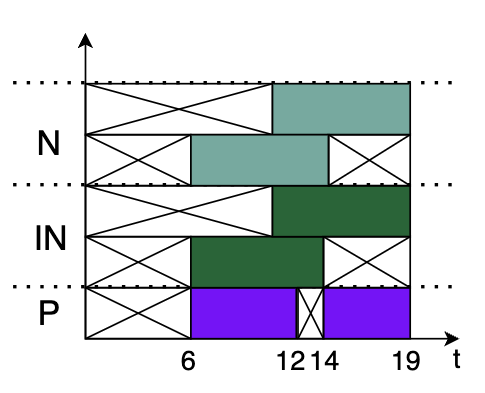
\includegraphics[width=0.20\textwidth]{images/calendars.png} }}%
    \caption{Running example of hospital process}%
    \label{fig:running_example}%
\end{figure*}
In this part, 
we first motivate our work with a real-life hospital
example. Then, we proceed to define the business
process scheduling problem (BPSP),
and lastly,
discuss the use of process mining for inference of BPSP parameters
from data.


\subsection{Motivating Example} We are motivated
by a hospital process 
that provides a sequence of treatments to cancer patients. 
The resources involved in the process, nurses (\act{N}), physicians (\act{P}), 
and infusion nurses (\act{IN}), are shared among patients 
and must be scheduled ahead of time. 
The duration of treatments varies significantly based on patient-specific context (e.g., patient complexity). 
Furthermore, the resources involved are not always available, as they follow specific shift schedules
and may go on planned vacations. For instance, 
nurses work 8 hours a day, 5 days a week, either in the morning or in the afternoon. Physician calendars are
highly variable, and depend on exogenous factors 
(e.g., physicians serving in multiple hospitals). 




The hospital process is depicted in Figure~\ref{fig:TPN}, which illustrates possible patient pathways. The activities are represented by white rectangles, and the time required to complete each activity is defined by probability distribution functions. The process begins with the \act{Blood Draw} activity, performed by a nurse (\act{N}), and continues with the parallel execution of the \act{Vitals} (for vital signs) and \act{Examination} activities, performed by a nurse and a physician (\act{P}), respectively. Finally, based on previous activities, the physician decides whether to proceed with \act{Chemo. Infusion}.

To complement the picture, Figure~\ref{fig:calendar} illustrates resource shifts for a typical day. Nurses have various shifts, which overlap for only two hours, between \act{11 am} and \act{2 pm}, while the physician has a two-hour break during which no \act{ examination} activity can be performed. The hospital processes approximately 1000 patients per day, involving over 5000 activities. The goal is to find a proactive schedule that probabilistically minimizes the global Makespan, e.g., the time that the last patient leaves cannot exceed \act{6PM} with probability of at least $0.95$. 

\subsection{Problem Definition} 
Referring to the definition in ~\cite{sanchez2023survey}, a case in a business process corresponds to a project, and the activities within the case map to the jobs that comprise the project. Business process scheduling problems (BPSPs) can therefore be represented using the following parameters\footnote{RCMPSP notation taken from~\cite{sanchez2023survey}.}: 
\begin{itemize}
    \item $\mathcal{I}$ is the set of cases enumerated by $i \in \{1, 2,....|\mathcal{I}|\}$,
    \item $A_i  = \{a_1, \ldots, a_{|A_i|}\}$ is the set of activities comprising case $i$, where $a_j, a_k$ may correspond to the same activity type (e.g., examination),
    and may repeat within a case,
    \item $\mathcal{A}$ is the set of all possible activity types, and $\phi$ is a mapping from activities to their types, $\phi(a_j) \in \mathcal{A}$,
    \item $\Pi_{i,a_j} \subseteq A_i$ represents activities that precede activity $a_j \in A_i$, i.e., their completion precedes the start of $a_j$,
    \item $\mathcal{R}$ is the set of resources involved in the process, with $r \in \{1, 2,....|\mathcal{R}|\}$, and
     $C_r$ being the capacity of $r$,
    \item $R_{i,a_j} \subseteq \mathcal{R}$ are the resources required to perform activity $a_j$ in case $i$, and $\rho(a_j) = R_{i,a_j}$ is a function that returns the set of resources required by an activity,
    \item $\mathcal{T} = \{0, 1, \ldots, T\}$ is a set of time periods (e.g., minutes) during a scheduling horizon of length $T$,
    \item $D_{i,a_j} \sim \mathcal{P}_{i,\phi(a_j), \rho(a_j)}$ is the number of time periods required to perform activity $a_j$ in case $i$, which follows the probability distribution $\mathcal{P}$ that depends on case $i$, activity type $\phi(a_j)$ and set of resources $\rho(a_j)$.\footnote{ The only stochastic components of BPSP are activity durations.}
    %$D_{i,a_j} \sim \mathcal{P}_{i,\phi(a_j), \rho(a_j)}$ is the (resource-, case- and activity type-dependent) \emph{random} number of time periods required to perform activity $a_j$ in case $i$, with $\mathcal{P}_{i,\phi(a_j), \rho(a_j)}$ being the distribution of the duration.\footnote{ The only stochastic components of BPSP are activity durations.} 
    \item $v_{r,t} \in \{0,1\}$ is the resource availability calendar, which is $1$ if resource $r$ is available at time period $t \in \mathcal{T}$.
\end{itemize} 
It is worth mentioning that the BPSP is a variation of the RCPSP that, 
to the best of our knowledge, has not yet been addressed in the scheduling literature~\cite{sanchez2023survey}.

Scheduling the business process is to assign each activity $a_j \in A_i,\ i=1,\ldots, |\mathcal{I}|,\ j=1,\ldots,|A_i|$ with a start time. Resource assignment is defined based on the activity requirement $R_{i,a_j}$, where non-interchangeable resources are treated as distinct.
%(resource assignment is implicit from the activity requirement $R_{i,a_j}$). 
Optimal scheduling in our setting is to find a schedule such that the 
latest completion time 
among all cases, i.e., the global Makespan $M$, is minimized. 



\begin{table}[t]
\resizebox{0.90\columnwidth}{!}{
    \begin{tabular}{c c c c c}
        \toprule
        \textbf{CaseId} & \textbf{Activity type}  & \textbf{Start} & \textbf{Complete} & \textbf{Resources} \\ 
        \midrule
        \act{1} & \act{Blood Draw} & \act{08:00} & \act{08:06} & \attr{N} \\
        \act{2} & \act{Blood Draw} & \act{08:01} & \act{08:07} & \attr{N} \\
        \act{3} & \act{Blood Draw} & \act{08:01} & \act{08:05} & \attr{N} \\
        \act{3} & \act{Vitals} & \act{08:05} & \act{08:11} & \attr{N} \\
        \act{2} & \act{Examination} & \act{08:07} & \act{08:14} & \attr{P} \\
        \act{2} & \act{Vitals} & \act{08:10} & \act{08:14} & \attr{N} \\
        \act{3} & \act{Examination} & \act{08:10} & \act{08:25} & \attr{P,N} \\
        \act{1} & \act{Vitals} & \act{08:11} & \act{08:14} & \attr{N} \\
        \act{1} & \act{Examination} & \act{08:11} & \act{08:30} & \attr{P,N} \\
        \act{2} & \act{Chemo. Infusion} & \act{08:20} & \act{09:10} & \attr{IN} \\
        \act{1} & \act{Chemo. Infusion} & \act{08:30} & \act{09:40} & \attr{IN} \\
        \bottomrule
    \end{tabular}
}
\caption{Example of a simple event log.}
\label{table:real_log_DT}
\end{table}



\subsection{Learning BPSP Parameters From Event Logs} 
If all parameters of the BPSP are at hand, one can immediately switch to solving the underlying problem.
However, if this is not the case, one can use historical data to infer these parameters with the use 
of process mining methods. 

Process Mining~\cite{van2016data} integrates data science with business process analysis to extract insights from event logs recorded by enterprise information systems, such as EPIC in healthcare~\cite{johnson2016comprehensive}. Event logs (see Table~\ref{table:real_log_DT}) provide a valuable source of data for learning the parameters required for scheduling problems. 
An event log consists of multiple cases, where each case 
is a sequence of events 
corresponding to the execution of a case, e.g., a single journey of a patient in a hospital. Each event 
in the sequence is a measurement of an activity and its characteristics. 
Specifically, events capture the type of activity, the resources involved and the start and end timestamps that define the duration of the activity.


\paragraph{Learning Activities and Precedence.} Activity types, which represent categories of activities performed in the process, are determined from the labels of activities recorded in the event log. Mapping these observed activities to predefined types involves grouping activities based on domain knowledge or textual similarity. The durations of activities can be derived from the start and end timestamps recorded in the event log. By analyzing these timestamps, probability distributions can be fitted to the observed durations of each activity type, such as normal or log-normal distributions, depending on the observed data, c.f.,~\cite{simod}. Precedence constraints can be inferred by examining the sequential order of activities in traces, identifying dependencies between activities where the completion of one activity consistently precedes the start of another~\cite{senderovich2019learning}. 

\paragraph{Inferring Resources and Capacities.} Resource capacities can be inferred by analyzing the frequency of resource usage over time, leveraging approaches such as \textit{SchedMiner}~\cite{SenderovichRGMM15}. 
The effective capacity is estimated by considering the maximum resource utilization observed in the event log. This estimate often serves as a tight lower bound, as there remains a small probability that some resources were available but never utilized.

%By determining peak resource utilization, capacity estimates act as lower bounds when full utilization is not observed in the log. 
Resource availability calendars can be constructed by analyzing the distribution of timestamps associated with resource usage, identifying periodic patterns such as daily or weekly schedules, which can be assumed constant over extended 
periods. Resource requirements for activities can be extracted from the resource identifiers associated with events in the log. 


\paragraph{Threats to Validity.} The application of process mining techniques relies on several assumptions. It is assumed that logs are complete, capturing all resources and activities involved in the process, and that activities are non-preemptive, meaning they run to completion once started. Resource capacities are assumed to remain fixed over time, with resources becoming available immediately after completing an activity, unless they are absent according to their calendar. Additionally, activity durations are assumed to follow a known distribution, and resource calendars are considered periodic and consistent over the given time horizon. All of these assumptions may be violated in practice. 

A first step in addressing threats to validity in process mining is to use representative event logs, i.e., logs that cover a time period meaningful to the process life-cycle and minimize the variability caused by seasonal behaviors. Variability in resource capacities and behaviors can be mitigated by estimating the capacity of pools of resources performing shared activities. Hence, resource pools reflect average performances and are not influenced by the behavior of individual resources. Finally, with respect to the
time perspective of the process, many state-of-the-art approaches replace predefined distributions with advanced statistical or machine learning models to more accurately capture process dynamics.


